\section{Inverter}

\subsection{Schematic}

Figure \ref{fig:inv_sch} shows the schematic of a inverter cell, including parameters for MOSFETs, designed from the previous laboratory session.

\begin{figure}[!htb]
	\centering
	\begin{subfigure}[b]{0.55\textwidth}
		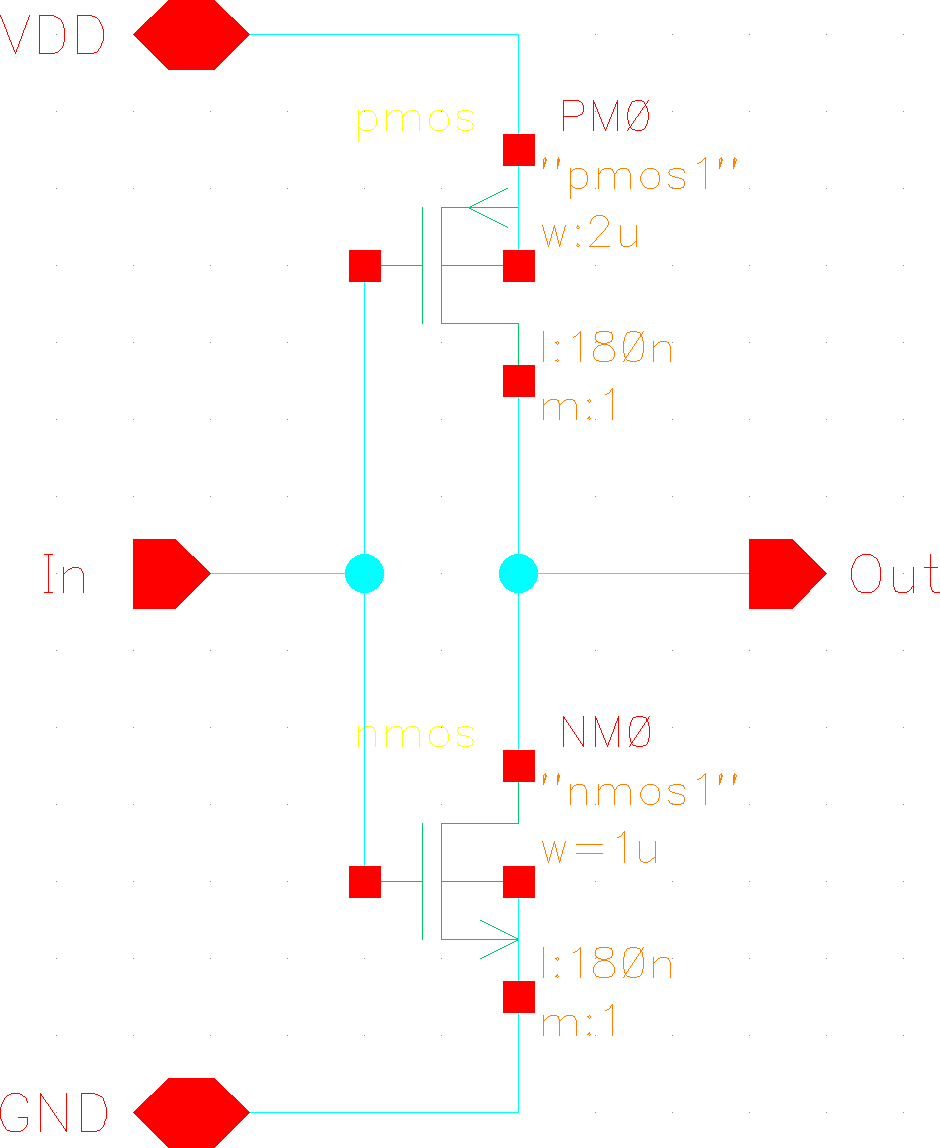
\includegraphics[width=\textwidth]{Inverter_sch}
		\caption{Schematic including MOSFET parameters}
		\label{fig:inv_sch}
	\end{subfigure}
	\begin{subfigure}[b]{0.3\textwidth}
		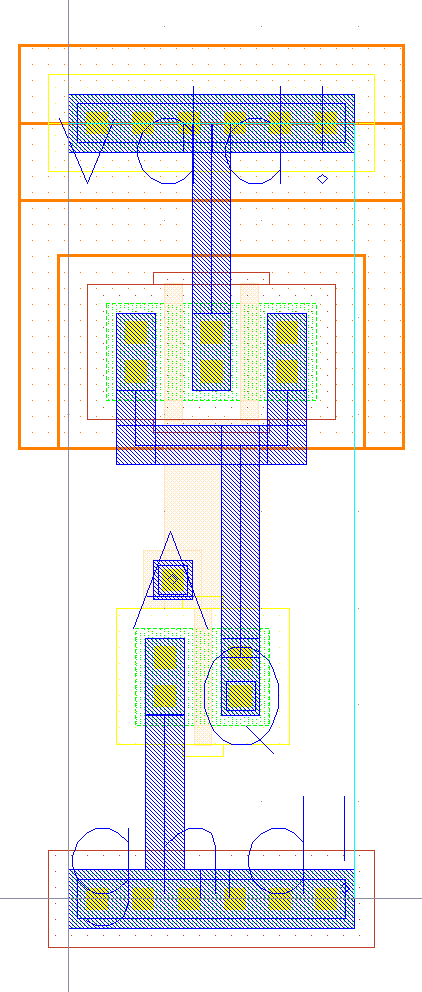
\includegraphics[width=\textwidth]{Inverter_lay}
		\caption{Final layout design}
		\label{fig:inv_lay}
	\end{subfigure}
	\caption{A inverter cell}
\end{figure}

\subsection{Layout}

Figure \ref{fig:inv_lay} shows the final layout designed for the inverter. The P-channel MOSFET (PMOS) is split into 2 fingers, to meet the height requirement for the standard cells ($8 \mu m$ in this case). The N-channel MOSFET (NMOS) and P-channel MOSFET (PMOS) are moved closer to the vertical centre, and $VDD$ is supplied to the centre tap of the PMOS instead, compare to the example layout given in laboratory notes. This is to accommodate the routing requirements at top and bottom spaces, used by the D-type Flip-Flop designed later.

To achieve minimum cell width, the spacing between cell boundaries to the left and right of the P+ implant inside the inverter PMOS should add up to the minimum value defined by the design rules, and kept the same across all standard cells. Therefore, when two standard cells are tightly placed next to each other, the design rule will not be violated, and no space will be wasted. The gpdk180 design rules shows the requirement is $0.4 \mu m$. Therefore, the spacing is determined to be $0.2 \mu m$ between the P+ implant and the cell boundaries.

The DRC and LVS verification were then executed, as shown in Figure \ref{fig:inv_vfy}. No DRC errors ensures the layout designed does not violate any design rules. LVS verification ensures the layout matches the schematic and parameters.

\begin{figure}[!htb]
	\centering
	\begin{subfigure}[b]{0.5\textwidth}
		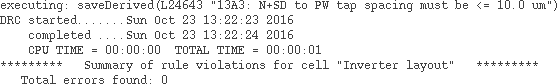
\includegraphics[width=\textwidth]{Inverter_drc}
		\caption{DRC checking result, no errors}
		\label{fig:inv_drc}
	\end{subfigure}
	\begin{subfigure}[b]{0.4\textwidth}
		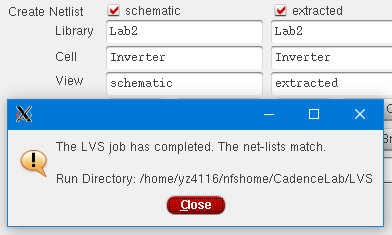
\includegraphics[width=\textwidth]{Inverter_lvs}
		\caption{LVS checking result, the extracted net-list matches the schematic}
		\label{fig:inv_lvs}
	\end{subfigure}
	\caption{Inverter cell layout verification}
	\label{fig:inv_vfy}
\end{figure}
